\documentclass{article}


\usepackage{arxiv}

\usepackage[utf8]{inputenc} % allow utf-8 input
\usepackage[T1]{fontenc}    % use 8-bit T1 fonts
\usepackage{hyperref}       % hyperlinks
\usepackage{url}            % simple URL typesetting
\usepackage{booktabs}       % professional-quality tables
\usepackage{amsfonts}       % blackboard math symbols
\usepackage{nicefrac}       % compact symbols for 1/2, etc.
\usepackage{microtype}      % microtypography
\usepackage{lipsum}
\usepackage{graphicx}
\usepackage{subcaption}

\title{A Scale-free topology construction model for Wireless Sensor Network (WSN)}


\author{
  Omprakash Sah Kanu \\
  Department of Computer Science \& Engineering\\
  National Institute of Technology Delhi \\
  Delhi 110040 (India)\\
  \texttt{151210051@nitdelhi.ac.in} \\
  %% examples of more authors
   \And
 Vaidya Srikar \\
  Department of Computer Science \& Engineering\\
  National Institute of Technology Delhi \\
  Delhi 110040 (India)\\
  \texttt{151210001@nitdelhi.ac.in} \\
  \And
   Dr. Richa Mishra\\
    Department of Computer Science \& Engineering\\
  National Institute of Technology Delhi \\
  Delhi 110040 (India)\\
  \texttt{richamishra@nitdelhi.ac.in} \\
}


\begin{document}
\maketitle

\begin{abstract}
WSNs have been an integral part of modern society and one of the most promising technologies of the future. They have been an important part in projects like smart cities, medical health, intelligent home, area surveillance, agriculture and military. However, research must address various challenges to help the widespread deployment of WSN. One of the major problems being faced by these networks is robustness. In this paper we have proposed an algorithm to generate scale-free WSNs. Scale-free networks have been widely known in complex networks for their robustness towards random failure. So adopting the concept of scale-free network and modifying it to suit various constraints of WSN has been the major part of our work in this paper. 
\end{abstract}


% keywords can be removed
\keywords{Wireless sensor network, Robustness, preferential attachment}


\section{Introduction}
A WSN contains group of spatially distributed sensor nodes deployed at a certain area of interest or dispersed randomly. The job of a sensor node is to sense the physical parameters of the area of deployment and route the data to a central location. The central location is usually a base station which act as a medium between the sensor nodes and the internet. 

Since the deployment of a node is dependent on the region of interest, each WSN shall have different node placements. Taking this factor into consideration we have made sure that our method work with random node deployment. We also took into consideration the coordinates where a particular node is placed at.    

A node is usually constrained with limited power supply, sensing range, processing power etc. The constraint power supply can lead a node to death if there is no external backup source. Failure of a node may also result due to human attacks or unfavourable environmental situtations such as fire or animal intervention. Failures may be random or malicious. In this paper we are concerned with random failures.

The main objective of our work is improving robustness of network topologies for WSNs. That means, we wanted to generate a network topology for any WSN deployment whereby the connection between as many nodes are preserved after certain nodes failure taking into consideration random failures where a attacker chooses a node randomly from the network and targets it. Thus, the resulting WSN toplogy with our method shall be resistant to random failure.

In our work, we chose scale-free topology. Scale-free has been adopted from the field of complex network theory. Scale-free networks research have shown its abundance in nature and man-made networks such as semantic network, protein-protein interaction, airline network, internet, WWW, software dependency graph, etc. All these networks strongly correlates with robustness to failure. The scale-free networks are also a good fit for homogeneous networks making it suitable for WSN with same radius of coverage and power-level. The main characterstic in a scale-free network is that its degree distribution follows a power-law. This means, in the scale-free network there is relative abundance of nodes with small degree than those with high degree. The high-degree nodes are called hubs. This means in a random attack, majority of small-degree nodes are more likely to be attacked whose failure doesn't affect the network connectivity. The generative model used for construction of scale-free topology has been Barab{\'a}si-Albert model, which has been modified to suit the WSN requirements. 

The remainder of the paper is organized as follows. In section 2, we present a brief overview of related works and literature survey. Section 3 describes our algorithm for scale-free topology construction. Section 4 shows evalution of our result and how it compares with other algorithms. Section 5 concludes this paper. Section 6 discuss our future work.

\section{Related-Work}

\section{Proposed algorithm}
In this section we shall brief on Barab{\'a}si-Albert model and how its been modified to suit WSN. Then we shall move ahead explaining our algorithm in detail.

BA model is an algorithm for generating random scale-free networks using preferential attachment mechanism. The algorithm was proposed by Albert Barab{\'a}si \& R{\'e}ka Albert to explain the existence of power-law in real networks. The algorithm works in the following way:
\begin{enumerate}
\item The algorithm begins with $m_o$ initial connected nodes.
\item The network grows by introducing new nodes to join the network one by one. 
\item The newly joined node connects to $m \leq m_o$ existing nodes with probability $p_i$ that is proportional to the number of links that the existing nodes already have. This step is called as preferential attachment. The probability $pi_i$ that a new node is connected to node $i$ is given as:
		\begin{equation}
		p_i = \frac{k_i}{\sum_i{k_j}}
		\end{equation}
where $k_i$ is the degree of node $i$ and the sum is made over pre-existing node $j$
\end{enumerate}
This method can be successfully used to generate scale-free networks with power-law distribution. But it has to be modified enough to suit the various constraints of WSN. The various constraints of WSN to be taken into account include: 
\begin{enumerate}
\item Communication range: A sensor node can only connect to a node $i$ in its radius of coverage $R$. Calling the nodes within $R$ to be neighbours of $i$. $i$ can only have preferential attachment with its neighbours. The length of $R$ needs to large enough to have enough neighbours for preferential attachment. Small $R$ cause very few neighbours which can result in small clusters in the network and thus fails to have scale-free property.
\item Degree size: The maximum degree that $i$ can have is required to be controlled. This is because, higher the degree of $i$, higer the number of nodes that passes data to $i$. Failing to control it can cause higher energy drainage. 
\item Network growth: WSN network can be static as well as dynamic. When dynamic, new nodes shall be introduced, they shall have preferential attachment with its neighbours. When static, the existing nodes need to wire themselves with $p_i$ within their neighbourhood.
\end{enumerate}

Taking above factors into consideration, our proposed algorithm for WSN is described below.

We begin by generating random coordinates in area $DXD$. Each coordinate denote the position of a node. Each node has radius of coverage $R$. We have considered homogeneous WSN keeping $R$ for each node same. Within $R$ we identify nodes that shall be called its neighbours $nbr$. 

We choose a node at the centre of network. Initially there are no edges between the nodes. So for $i$ we randomly choose a node $j$ from $nbr$ and make a edge between them. Else, we define the connection probability for nodes in $nbr$, $p_i$ as follows. If degree of $i$ is less than highest degree $HD$ then \begin{equation} p_i = \frac{k_i}{\sum_i{k_j}}\end{equation} else, \begin{equation}p_i = \frac{k_i}{k_i*\sum_i{k_j}}\end{equation} $HD$ is choosen such that to limit highest degree within the network. Equation 2 is similar as equation 1 if degree of a node is less than $HD$ else equation 3 is used to reduce the probability of choosing the node.

After a node $i$ chooses and makes connection with a node $j$ in its $nbr$ with probability $p_i$, we choose $j$ as next node. Next, node $j$ chooses a node from its $nbr$ and make connection with it. The process follows until $e \leq e_{max}$ connections are made. $e_{max}$ is the total possible edges that is possible for $N$ nodes, mathematically defined as $e_{max} =  \frac{N*(N-1)}{2}$ and $e$ is the fraction of edges of $e_{max}$.


\section{Results}
In this section we shall evaluate the scale-free property our model and then analyse its robustness. The alogorithm was implemented and simulated using Python on Spyder.

We took an area of $500*500 m^2$ and randomly choosed $N$ coordinates within it. Each $N$ coordinates denote $N$ individual sensor-nodes deployed in its area of interest or distributed randomly. Each sensor-node were considered homogeneous with radius of coverage i.e. radius within which a particular sensor-node can send and recieve data with other nodes to be $R=200$. We choosed this number for our simulation purpose. $R$ is required to be choosen smartly by the deployer taking into consideration energy consumption ($R\propto E$) and number of neighbours for each node (less neighbours fail to form scale-free topology). We choose $m=1$ i.e. number of connections a particular node form during its turn to form preferential-attachment. We choosed number of edges for the network $e$ to be $0.01\%$ of $e_{max}$. $e$ is to be choosen considerably since large $e$ shall result in large number of nodes to have high degree, which shall reduce power efficiency of the network.

\subsection{Scale-free evaluation}
Figure 1 shows scale-free properties of the networks for our simulation. We have choosen three networks with different number of nodes thus different densities. We have presented two figures for each type of network. Top figure shows the actual network formation and bottom figure shows the degree distribution graph for the network. In the top figure, it can be noticed that there are two colors for the nodes - bright red and dark red. Bright red represents the hub nodes i.e. the nodes with higher degree and dark red represents nodes with low degree. 

For figure 1(a) has 100 nodes, figure 1(b) has 400 nodes and figure 1(c) has 800 nodes. It can be noticed that in the top figures the number of bright red nodes is considerably small as compared to dark red nodes. This means there are very few hubs in the network and large number of nodes with low degree. Same results are shown by the bottom graphs as well. In the graph x-coordinate shows degree size of the nodes and y-coordinate shows number of nodes having the particular degree. Notice that, for higher degree the count of nodes are less while for smaller degree the count of nodes are higher.

This proves that our proposed algorithm for generating scale-free network topology, which has been simulated in figure 1, indeed generates scale-free topology.

\subsection{Robustness analysis}


\begin{figure}[!htb]
	\minipage{0.32\textwidth}
	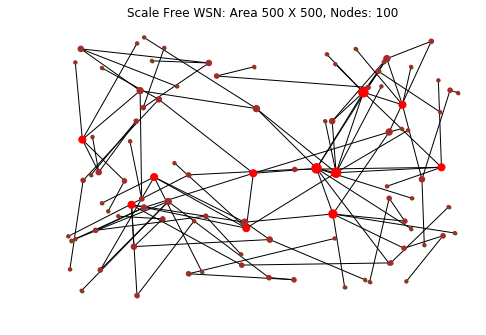
\includegraphics[width=\linewidth]{Results/100-1.png}
	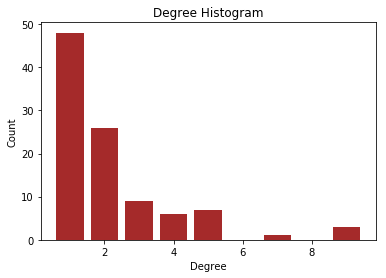
\includegraphics[width=\linewidth]{Results/100-1(B).png}
	\begin{center}
		(a)
	\end{center}
	\endminipage\hfill
	\minipage{0.32\textwidth}
	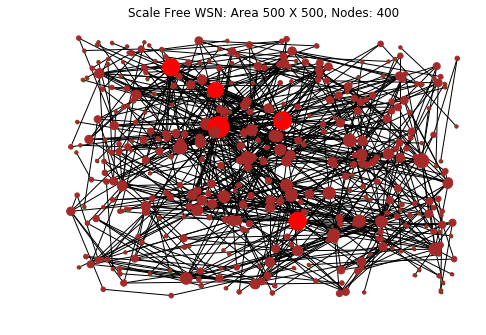
\includegraphics[width=\linewidth]{Results/400-1.png}
	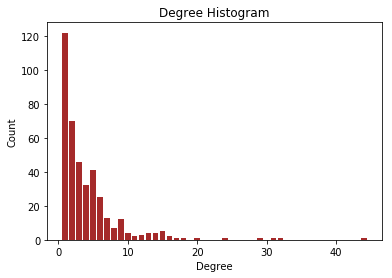
\includegraphics[width=\linewidth]{Results/400-1(B).png}
	\begin{center}
		(b)
	\end{center}
	\endminipage\hfill
	\minipage{0.32\textwidth}%
	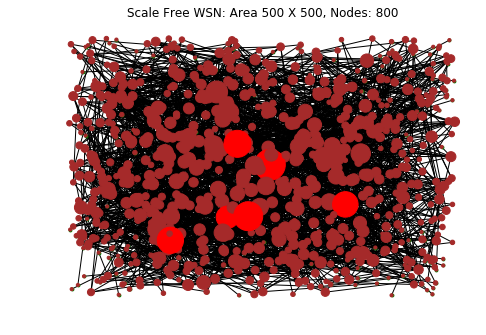
\includegraphics[width=\linewidth]{Results/800-1.png}
	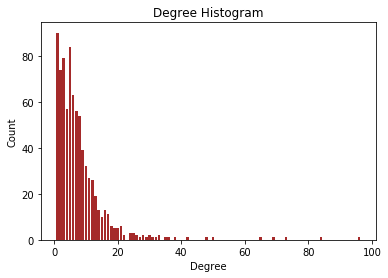
\includegraphics[width=\linewidth]{Results/800-1(B).png}
	\begin{center}
		(c)
	\end{center}
	\endminipage
	\caption{Scale-free properties in WSNs. For each figure R=200, m=1, area: 500x500 (a) N=100 (b) N=400 (c) N=800}
\end{figure}

\begin{figure}[!htb]
	\minipage{0.32\textwidth}
	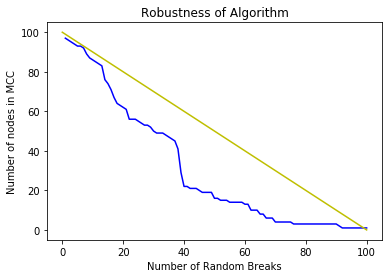
\includegraphics[width=\linewidth]{Results/100-1(G).png}
	\begin{center}
		(a)
	\end{center}
	\endminipage\hfill
	\minipage{0.32\textwidth}
	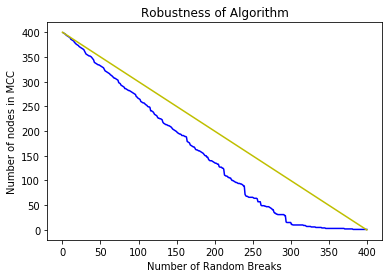
\includegraphics[width=\linewidth]{Results/400-1(G).png}
	\begin{center}
		(b)
	\end{center}
	\endminipage\hfill
	\minipage{0.32\textwidth}%
	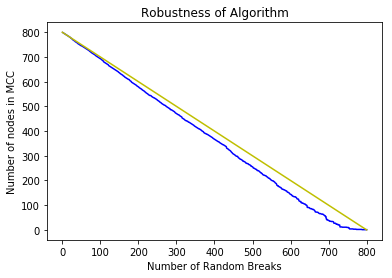
\includegraphics[width=\linewidth]{Results/800-1(G).png}
	\begin{center}
		(c)
	\end{center}
	\endminipage
	\caption{Robustness results. For each figure R=200, m=1, area: 500x500 (a) N=100 (b) N=400 (c) N=800}
\end{figure}

\section{Conclusion}

\section{Future Works}


\bibliographystyle{unsrt}  
%\bibliography{references}  %%% Remove comment to use the external .bib file (using bibtex).
%%% and comment out the ``thebibliography'' section.


%%% Comment out this section when you \bibliography{references} is enabled.
\begin{thebibliography}{1}

\bibitem{kour2014real}
George Kour and Raid Saabne.
\newblock Real-time segmentation of on-line handwritten arabic script.
\newblock In {\em Frontiers in Handwriting Recognition (ICFHR), 2014 14th
  International Conference on}, pages 417--422. IEEE, 2014.

\bibitem{kour2014fast}
George Kour and Raid Saabne.
\newblock Fast classification of handwritten on-line arabic characters.
\newblock In {\em Soft Computing and Pattern Recognition (SoCPaR), 2014 6th
  International Conference of}, pages 312--318. IEEE, 2014.

\bibitem{hadash2018estimate}
Guy Hadash, Einat Kermany, Boaz Carmeli, Ofer Lavi, George Kour, and Alon
  Jacovi.
\newblock Estimate and replace: A novel approach to integrating deep neural
  networks with existing applications.
\newblock {\em arXiv preprint arXiv:1804.09028}, 2018.

\end{thebibliography}


\end{document}
